% Uses a slightly modified IEEE VGTC template in conference mode
\documentclass{vgtc}
\usepackage{times}
\usepackage[pdftex]{graphicx}

\usepackage[utf8]{inputenc}
\usepackage[T1]{fontenc}
\usepackage{tikz}
\usepackage{algorithm}
\usepackage{algpseudocode}
\usepackage{pifont}

\usepackage{tree-dvips}
\usepackage{qtree}
\usepackage{tikz-qtree}
\usepackage{etoolbox}
\usepackage{pgfplots}
\usetikzlibrary{calc}


% If submitting a paper to a conference for review with a double
% blind reviewing process, replace the value ``0'' below with your
% OnlineID. Otherwise, leave it at ``0''.
\onlineid{0}

\vgtccategory{Research}

\usepackage{url}

%% Paper title.
\title{A modular GPU raytracer using OpenCL for non-interactive graphics}

\author{Henrique Nunes Jung\thanks{e-mail: henriquenj@gmail.com}
\and Vinicius Jurinic Cassol\thanks{e-mail: vjcassol@unisinos.br}}
\affiliation{\scriptsize Universidade do Vale do Rio dos Sinos}


%% Abstract section.

\abstract{

  We describe the development of a modular plugin based raytracer
  renderer called \emph{RenderGirl} suitable for running inside the
  OpenCL framework. We aim to take advantage of heterogeneous
  computing devices such as GPUs and many-core CPUs, focusing on
  parallelism. We implemented the traditional partitioning scheme
  called \emph{bounding volume hierarchies}, where each scene is
  hierarchically subdivided into axis-aligned bounding boxes, so a ray
  may only need to traverse a subset of geometry by traversing the BVH
  and discarding objects it surely cannot hit, optimizing the
  rendering process. These structures were implemented on a many-core
  high parallel architecture suitable for OpenCL, which needed a
  specific binary tree structure implementation ready for stackless
  traversal on GPUs. RenderGirl is split between two main portions:
  Core and Interface, where the Core portions provide the bulk of
  ray-tracing operations and manage the communication with OpenCL; and
  the interfaces provide communication with a given host program,
  seeking modularity. In this paper we describe our results and
  performance gains with our partitioning scheme.

\smallskip

\noindent \textbf{Keywords:} GPGPU, OpenCL, computer graphics, raytracing
} % end abstract

\begin{document}

\firstsection{Introduction}

\maketitle

Platforms for general purpose computing using GPUs started when
NVIDIA\footnote{NVIDIA website \url{http://www.nvidia.com/}} released
its GPGPU platform called CUDA\footnote{CUDA homepage
 \url{http://www.nvidia.com/object/cuda_home_new.html}}, which is
capable of running only on NVIDIA hardware. OpenCL\footnote{OpenCL on
 Khronos Group website \url{https://www.khronos.org/opencl/}} was
born sometime later using the label \emph{heterogeneous computing}, in
order to specify that the platform was supported by many kinds of
hardware and computer processors, including CPUs and non-NVIDIA GPUs,
which could be implemented by any vendor interested in developing
hardware focused on parallel computation.

Within this context, this work aims to provide a modular plugin-based
raytracer software that takes advantage of the parallel capabilities
of modern GPUs while maintaining hardware agnosticism by using the
portability OpenCL provides to hardware vendors and developers. By
being modular, it's also capable of running inside larger 3D suites
such as Blender, this way we can delegate other tasks to the host 3D
program and focus on the rendering tasks. We developed a C++
application and a reference plugin for Blender, used to validate this
architecture. The code has only portable system calls and OpenCL
function calls.

Intrinsic problems that arrive with GPU ray tracing include the cost
of synchronizing and stopping working threads, poor branch prediction,
high latency of different OpenCL memory models, high latency on the
bus used between GPU and main memory (usually PCI Express) and the
broad variety of GPUs and OpenCL capable hardware, which can generate
different results on different setups. It also cannot have complex data
structures such as dynamic arrays and linked lists.

There are several acceleration structures meant to increase the efficiency
of rendering, which are called \emph{spatial data structures}. Some of
these structures are \emph{bounding volume hierarchies} (BVH),
\emph{binary space partitioning}, trees, quad-trees and octrees. They
hierarchically subdivide a scene so that the queries for their objects
become faster \cite[Chapter~14.1]{akenine-moller:2008}. Non real-time
renderers do not have time constraints and therefore can employ
expensive algorithms, generating images of higher quality. They can also
take advantage of spatial structures in order to speed up
operations. For RenderGirl, we developed a variant of the BVH
partitioning structure suitable for stackless traversal on the GPU.


Our contributions include:

\begin{itemize}
  \item A renderer independent of a given 3D software.
  \item A raytracer designed to take advantage of parallel
    computation capabilities of modern GPUs and other OpenCL-capable
    devices.
  \item A modular architecture with replaceable components that
    communicates with a known interface.
  \item Usage of acceleration structures suitable for storing scene
    information inside OpenCL architecture.

\end{itemize}

\section{Related Work}
\label{sec:related-work}

Applications that provide GPU rendering capabilities for
non-interactive graphics include Blender Cycles\footnote{Cycles
  website \url{http://www.blender.org/manual/render/cycles/}} , Octane
render \footnote{Octane website
  \url{https://home.otoy.com/render/octane-render/}}, V-Ray renderer
\footnote{VRAY website
  \url{http://www.chaosgroup.com/en/2/vray.html}}, Redshift
\footnote{Redshift website
  \url{https://www.redshift3d.com/products/redshift}} and Indigo
renderer \footnote{Indigo website
  \url{http://www.indigorenderer.com/}}. Indigo and Cycles both claim to
run using the OpenCL framework. Cycles is the only one that is free
software; originally it only supported CUDA-capable devices, but newer
versions of Blender ship with Cycles that works with limited features
also on OpenCL, although the developers specify that the CUDA platform
is more mature \footnote{Cycles GPU rendering page
  \url{http://www.blender.org/manual/render/cycles/gpu_rendering.html}}.
Cycles also takes a different approach for device abstraction by
performing \emph{platform abstraction} by issuing commands to a common
\emph{device interface} that can redirect function calls to CUDA,
OpenCL, CPU or network; although the latter is still experimental
\footnote{Blender Cycles Developer Documentation
  \url{http://wiki.blender.org/index.php/Dev:2.6/Source/Render/Cycles/Devices}}. Our
work delegates the device abstraction entirely to OpenCL.

NVIDIA developed a framework called NVIDIA OptiX \footnote{OptiX
  website \url{https://developer.nvidia.com/optix}} which is intended
to be a general purpose ray tracing engine designed for NVIDIA GPUs
and other many-core architectures. It can be used for a variety of
tracing-based algorithms and also on domains beyond computer graphics
such as sound propagation, collision-detection and artificial
intelligence. They aim to provide a set of programmable operations for
implementing ray tracing operations, in a pipeline model comparable
with OpenGL and Direct3D \cite{Parker:2010:OGP:1778765.1778803}.

Recent related work on the computing literature includes: Áfra and
Szirmay-Kalos propose a novel traversal algorithm for BVH that doesn't
use a stack, and can be executed both on CPU and GPU platforms. They
introduce the concept of \emph{bitstack}, which is an integer used in
the place of a stack \cite{Afra}. Kalajanov and colleagues propose an
acceleration structure using hierarchical two-level grids implemented
in CUDA, which can eliminate problems arriving from using a single
uniform grid for subdividing a scene. They call it the "teapot in a stadium"
problem, where a great amount of objects is allocated on a single
cell of the uniform grid \cite{Kalojanov}. Ravichandran and colleagues
propose a parallel divide and conquer raytracing suited for
GPUs. Divide and conquer ray tracing removes the need of creating an
explicit acceleration structure once per frame, instead it creates an
approximation using bound boxes \cite{Ravichandran}. Shumskiy and
Parshin write a comparative study of ray-triangle intersection
algorithms, how they perform on GPU hardware and how BVH acceleration
structures can be optimized for each one. They point out that some of
their results differ from generation to generation of the same line
of GPUs due to changes in the micro-architecture.
% TODO: this last sentece should go to another section, more specific
\cite{Shumskiy}. Wong and colleagues propose an optimization method for
GPU ray tracing by dividing objects into view-sets based on light and
camera position, the BVH is then built using these views-sets, this
way the amount of triangles on the BVH is reduced \cite{Wong}. Widmer
and colleagues propose efficient acceleration structure for real-time
screen space raytracing, they use a hybrid data structure combining
BVH and local planar approximation \cite{Widmer}. A great portion of
these works deal with acceleration structures for GPU raytracing -
e.g. kd-trees, BVHs -, which indicates the complexity of these
structures on GPU hardware.


\subsection{Contextualization}

Our own implementation relies on the ray-triangle intersection algorithm
developed by Möller and Trumbore that aims to be fast by avoiding
ray-plane intersections\cite{moller}.

While the software is intended to work on all hardware capable of
running OpenCL, we tried to focus on GPUs, so optimization for this
type of processor received preference. It's also worth noting that
this work does not have real-time constraints and it is designed to be
used as an \emph{offline} raytracing, so image quality is more
important than rendering times.

Our work differs from the previously mentioned publications by
focusing on modularity and portability, both of hardware and operating
system.

\section{Methodology}
\label{sec:methodology}

We developed a GPU raytracer using the OpenCL framework called
\emph{RenderGirl}\footnote{RenderGirl project page
  \url{https://github.com/henriquenj/rendergirl}} licensed under LGPL.
We try not to pose any restriction on the use of the software
regarding its host program, so anyone can implement their own
interfaces.

Most of the code is written using C++, with small portions
written in Python and OpenCL C. Tools used in the development include
Visual Studio for project files and compilation under Windows and Git
for source control.

The host program of RenderGirl is Blender, which provides all the base
functionality of a 3D software suite. RenderGirl connects with Blender
through its Python API and implements a \emph{RenderEngine}
interface. The host software performs all communication with the final
user through its own GUI.

The software can also run as a standalone executable file through its
command-line interface. This interface has minimum dependencies and
does not output any files, it just reports if the rendering was successful.

We try not to implement features that are not intrinsically related with
rendering, so RenderGirl delegates other tasks to the host program as
much as possible. This includes the loading of 3D models, user interface
interactions, image presentation and image saving. We believe this is the
most useful and optimized way to solve the problem at hand.

\section{Architecture}
\label{sec:architecture}

RenderGirl is composed of a \emph{core} that communicates with a given
\emph{interface}. The overall architecture is depicted at figure~\ref{fig:architecture}. Each of these components has a specific set
of tasks inside the program.

The core portion is a static library that provides an API for
receiving the 3D scene structure - vertices, triangles, objects,
cameras and lights - and the OpenCL device selection. It performs all of the
communication between OpenCL and the interfaces, handling its
context. The output of the render is an array of pixels with the
rendered frame. The core also provides the Log Subsystem dedicated to
log operations. Most of the interactions with the raytracer occur
using a shared object called \emph{RenderGirlShared}, which is
implemented as a shared singleton. Scene structures are managed by a
singleton called \emph{SceneManager}, providing an API for setting up
a scene using RenderGirl data structures; it's also responsible for
subdividing the scene into BVH structures and making it suitable for
OpenCL memory models.


The interfaces can be anything from executables to dynamic libraries,
depending on the plugin interface provided by the host 3D
program. Interfaces link themselves to the core at compile time and translate
all the requests from the host program. They can pick individual
features to support, and a given interface may support only a subset
of features of the core. Three interfaces are provided as examples,
they are:

\begin{itemize}
\item \emph{Console interface}: The simplest interface. It is linked to
  the core and compiles as an executable. It only provides options for
  OBJ loading and does not output any image file. It's useful for
  porting the Core to other platforms and making sure it's working.
\item \emph{wxWidgets interface}: compiles as a standalone
  application with a GUI for loading OBJ files and render models,
  using the wxWidgets\footnote{wxWidgets website
    \url{http://wxwidgets.org/}} toolkit. The user can choose
  attributes of the scene like camera position, color of light source
  and the output image format. It's likely to be deprecated over the
  Blender plugin interface due to the amount of dependencies it
  carries.
\item \emph{Blender Plugin}: the Blender plugin is the interface we
  provide as reference design to other interfaces for RenderGirl.
\end{itemize}

The core API is designed to only have synchronous calls, so each
function call will block the program - including the rendering
function which can take several minutes to complete. The reasoning
behind this is that every host program will provide different
asynchronous APIs for its plugin system in a different manner (or even won't
provide it at all) so we don't want to impose an asynchronous model at
this stage of development, leaving it for the interfaces to implement
their own. As an initial design decision to ease portability, the core
contains no system-dependent calls apart from OpenCL itself.

\begin{figure}
\centering
\usetikzlibrary{positioning,calc,fit}

\definecolor{black_red}{RGB}{179,0,0}
\definecolor{black}{RGB}{0,0,0}
\definecolor{blue}{RGB}{0,51,153}
\definecolor{orange}{RGB}{255,128,0}


\pgfdeclarelayer{core}
\pgfdeclarelayer{runtime}
\pgfsetlayers{core,main}

\pgfkeys{
  /tikz/node distance/.append code={
    \pgfkeyssetvalue{/tikz/node distance value}{#1}
  }
}

\newlength\myframesep
\setlength\myframesep{0pt}

\newcommand\widernode[5][core_node]{
\node[
        #1,
        inner sep=0pt,
        shift=($(#2.south)-(#2.north)$),
        yshift=-\pgfkeysvalueof{/tikz/node distance value},
        fit={(#2) (#3)},
        label=center:{\color{white}#4}] (#5) {};
}
% fix widernodeabove function, right now will shift nodes on X axis
\newcommand\widernodeabove[5][core_node]{
\node[
        #1,
        inner sep=0pt,
        shift=($(#2.north)+(#2.north)$),
        yshift=+\pgfkeysvalueof{/tikz/node distance value},
        fit={(#2) (#3)},
        label=center:{\color{white}#4}] (#5) {};
}

\begin{tikzpicture}[node distance=3pt,outer sep=0pt,
core_node/.style={
  draw=black,
  fill=black_red,
  rounded corners,
  font={\color{white}},
  align=center,
  minimum width = 70pt,
  text height=12pt,
  text depth=6pt},
other_node/.style={
  fill=black,
  draw=black,
  rounded corners,
  font={\color{white}},
  align=center,
  minimum width = 60pt,
  text height=12pt,
  text depth=6pt},
interface_node/.style={
  fill=orange,
  draw=black,
  rounded corners,
  font={\color{white}},
  align=center,
  minimum width = 70pt,
  text height=12pt,
  text depth=6pt},
host_node/.style={
  fill=black,
  draw=black,
  rounded corners,
  font={\color{white}},
  align=center,
  minimum width = 216pt,
  text height=12pt,
  text depth=6pt},
]

% core nodes

\node[core_node] (log) {Log subsystem};
\node[core_node, right=of log] (scene) {Scene Manager};
\node[core_node, right=of scene] (shared) {RenderGirl shared};
\widernode{log}{scene}{OpenCl wrapper}{wrapper};
\node[core_node, below=of shared] (kernels) {Kernels};

% interface

\node[interface_node, above=of scene](wrapper_host){Host structures};
\node[interface_node, above=of log](listeners){Log Listeners};
\node[interface_node, above=of shared](flow){Flow control};

\begin{pgfonlayer}{core}
\draw[core_node,draw=black,fill=black_red!40]
 ([xshift=-\myframesep,yshift=3\myframesep]current bounding box.north west)
    rectangle
  ([xshift=\myframesep,yshift=-\myframesep]current bounding box.south east);
\end{pgfonlayer}

% opencl runtime nodes

\widernode[other_node]{wrapper}{wrapper}{OpenCL runtime driver}{runtime}
\node[other_node, below=of kernels](compiler){OpenCL Compiler};

%  hardware

\widernode[other_node]{runtime}{compiler}{Hardware}{hardware}

% host 3d software

\node[host_node, above=of wrapper_host](host){Host 3D software};

\end{tikzpicture}
\caption{Architecture of RenderGirl. Red represents core components,
  orange represents interface components. Black represents third party
  components.}
\label{fig:architecture}
\end{figure}

\subsection{Blender Plugin}

We implemented a Blender plugin, which effectively made Blender our
host 3D program for all our tests. Having it within a major 3D program
is useful since it provides many interesting facilities, such as 3D
model loading.

Blender does not expose a C/C++ API for its extensions, so we had to
use the Python API instead. This raised the question of how we could
connect the RenderGirl C++ API with the Python side. Several solutions
were considered. One approach is to use the C Python
API\footnote{Python C API manual
  \url{https://docs.python.org/3.5/c-api/}} within a wrapper interface
module for RenderGirl, this approach was deemed too complex since it
would require the addition of a compile-time dependency with Python, it
would also tie our version of Python to Blender's version, likely
breaking compatibility when Blender decided to change its own
version. Another approach was to use Swig\footnote{Swig website
  \url{http://www.swig.org/}} for automatic wrapper generation, this
option also has the downside of adding a compile time dependency and an
extra build step.

The solution we ultimately chose was to compile a small C wrapper
around the RenderGirl core into a shared library. With a pure C
interface, we then used a Python module called ctypes\footnote{ctypes
  reference \url{https://docs.python.org/3.5/library/ctypes.html}},
which can load shared libraries and execute C functions loaded from
it. It provides support for callbacks - used on the log subsystem -
and all basic C types. With this approach there's no new dependencies
and no actual Python reference on the compiled Blender interface. We
can also reuse it on a future plugin from another host program if it
supports a C API.

There's still a portion written in Python, mostly the conversion of
data types and user interface additions to Blender. The major
difference between the data from both programs is that Blender
interprets the Y axis as depth instead of height. We also make use
of triangulation features of Blender, to make the scene compatible
with RenderGirl.

\subsection{OpenCL scheduling model}

OpenCL dispatches each execution of the raytracer by running a piece of
code called \emph{kernel}. Each kernel runs once inside a
\emph{work-item} which belongs to a \emph{work-group}. The exact
nature of the execution will be hardware dependent - e.g. a work-item
can become a thread -, we assume that each work-item can work
independently with no knowledge of other work-items, and therefore the
kernels do not perform any synchronization.

We launch one work-item executing one kernel per pixel of the
image. Each kernel will then build a ray based on pixel location
within the image to be tested for collision against the BVH structure,
where each ray may reach a leaf node, in which case it must test
against all the geometry of that object. This approach works well in
parallel because it does not require any synchronization among
work-items, hence it's well suited for GPUs.


\subsection{Scene structures}

In order to make a 3D scene fit into an OpenCL compatible structure,
we must not rely on complex data structures such as linked lists and
dynamic arrays. Pointers can only be used with a feature called
\emph{shared virtual memory}, however it's only available on OpenCL
2.0, and NVIDIA still has its implementation running on 1.2, so we
didn't want to rely on SVM.

Figure~\ref{fig:data-org} shows how the 3D geometry is organized
within the target device. The structure is similar to the OBJ file
format. The core concept are the \emph{global buffers}, they
collectively describe the geometry of the entire scene. E.g. the
vertices buffer contains all vertices for the entire scene. The vertex
buffer is indexed by the triangle buffer. The triangle buffer is then
divided into regions that compose the objects. An object's metadata
array describes where each object starts on the triangle buffer and
where it ends. The triangle buffer is usually provided by the host
program, so we must sanitize it to make sure it does not point past
the end of the vertices array.

\begin{figure*}
\centering

\includegraphics[width=1.0\textwidth]{data-organization.png}
\caption{The relationship of each data buffer that composes the
  geometry within the OpenCL device. Dotted arrows represent an
  integer index that points to some other array. The BVH will be
  covered in its own section.}
\label{fig:data-org}
\end{figure*}


\subsection{Acceleration structures}

Acceleration structures are commonly used on ray tracing in order to
avoid expensive and inefficient brute-force ray-triangle intersection
tests for the entire scene. With these structures, using a given ray,
we can query for only a subset of triangles and perform the
intersection tests on them.

Thrane and Simonsen conduct a study comparing three different
acceleration structures and their implementations on GPUs: bounding
volume hierarchies, kd-trees and uniform grids. On their experiments,
they concluded that BVH outperforms the other two except for a few
cases, citing the simpler nature of the traversal code with minimal
branching as the most likely responsible for the good results
\cite{Thrane}. After careful consideration of their results, we chose
BVH for our own implementation.

The process of using acceleration structures is usually divided in two
steps: \emph{construction} and \emph{traversal}. The BVH was
originally proposed by Kay and Kajiya\cite{kay1986ray}, they describe
an implementation using convex hulls as bounding volumes for each level
of the tree.

For our BVH in GPU, the \emph{construction} portion is roughly the
same as described by Kay and Kajiya. The BVH is built as a binary tree
where at each level objects are sorted by their absolute position
either in the X or Y axis, the collection of objects is then split into
half, composing the two children of that node. The axis used for
ordering are swapped at each level of the tree in an attempt to make a
fair distribution of objects. This process of ordering and division
repeats itself until the collection of objects is reduced to one, making it a
leaf node, which then contains all the geometry of that particular
object. The major difference between our approach is that we use
\emph{axis-aligned bounding boxes}(AABB) as bounding volumes instead of
convex hulls, since the traversal code is less complex, although with
a much less tightly fit bounding volume. Thrane and Simonsen mention
that there's a great penalty of running complicated code on the
GPU\cite{Thrane}. Every node holds an AABB fitting all the geometry of
its child nodes, so a ray must only test a collision against the AABB,
if the collision fails, the algorithm can discard that sub-tree and
resume processing on the next sibling node. If the program reaches a
leaf node, then the ray must be tested against all the geometry of
that object within the leaf node. All the construction phase happens
on the CPU.

On the \emph{traversal} step, we implemented the traversal algorithm
described by Thrane and Simonsen in their master
thesis\cite{Thrane}. The main problem to be solved here is to overcome
the lack of stacks on GPU hardware, since tree traversal algorithms are
usually implemented using recursion. The key difference from
traditional CPU implementations is that we build a fixed-order
\emph{traversal array} on the CPU and only iterate over it in the GPU,
so we never transmit the tree to the OpenCL device but rather the
iteration itself. The traversal array already contains the nodes we
must intersect in the correct order. The BVH node on the traversal
array has three properties: the AABB that fits all the geometry of
that node and its children, the \emph{escape index} and an index that
points to an object in the global list of objects. The escape index
represents the index where the traversal should resume if the current
node's AABB fails to intersect with the ray. If the traversal should
end, the escape index is equal to the size of the traversal array,
acting as a global escape index. This can be visualized on
figure~\ref{fig:bvh}. The object index is only valid in child nodes,
and it's flagged as -1 when in a middle node. The traversal is done in
a top-bottom left to right order. The algorithm for traversal is
detailed on Algorithm~\ref{alg:bvh-traversal}.


\begin{algorithm}
\caption{BVH traversal on OpenCL device}
\label{alg:bvh-traversal}
\begin{algorithmic}[1]
\State Given a ray $r$
\State $tarray\gets$ The traversal array
\State $s\gets$ size of traversal array
\State $index\gets 0$
\While{$index < s$ }
\State $node\gets$ element from $tarray$ at $index$
\If{$r$ intersects with $node$'s AABB}
\If{$node$ is a leaf node}
\State Executes ray-triangle intersection with all triangles on this leaf node and return the nearest
\Else
\State $index\gets$ $index$ + 1
\EndIf
\Else
\State $index\gets$ $node$'s escape index
\EndIf
\EndWhile
\end{algorithmic}
\end{algorithm}

This implementation is a little bit different than Thrane and Simonsen
because they implemented the ray-traversal in several passes, where
the control goes back to CPU, so they must retain intermediate
renderer states and hit records. This approach is probably due to
memory constraints at the time the implementation was done. Our
rendering happens by enqueuing a single OpenCL kernel only once, and
the control does not go back to the CPU until the frame is formed.

\begin{figure}
\centering
\newrobustcmd*{\square}[1]{\tikz{\filldraw[draw=#1,fill=#1] (0,0)
rectangle (0.2cm,0.2cm);}}

\newrobustcmd*{\mycircle}[1]{\tikz{\filldraw[draw=#1,fill=#1] (0,0) circle [radius=0.1cm];}}

\newrobustcmd*{\mytriangle}[1]{\tikz{\filldraw[draw=#1,fill=#1] (0,0) --
(0.2cm,0) -- (0.1cm,0.2cm);}}

\begin{tikzpicture}[sibling distance=20pt]
\tikzset{level distance=30pt}
\Tree[.\node(0){0}; [.\node(1){1}; [.\node(2){2}; \mytriangle{red}A ]
               [.\node(3){3}; \mytriangle{red}B ]]
          [.\node(4){4}; [.\node(5){5}; \mytriangle{red}C ]
                [.\node(6){6};
                [.\node(7){7}; [.\node(8){8}; \mytriangle{red}D ][.\node(9){9}; \mytriangle{red}E ]]
                [.\node(10){10}; [.\node(11){11}; \mytriangle{red}F ]
                [.\node(12){12}; \mytriangle{red}G ]]]]]
\node [anchor=base, right=14em]  (13) {13};
\draw[semithick,dashed,->] (1.east) to (4.west);
\draw[semithick,dashed,->] (2.east) to (3.west);
\draw[semithick,dashed,->] (3.east) to (4.west);
\draw[semithick,dashed,->] (5.east) to (6.west);
\draw[semithick,dashed,->] (7.east) to (10.west);
\draw[semithick,dashed,->] (8.east) to (9.west);
\draw[semithick,dashed,->] (7.east) to (10.west);
\draw[semithick,dashed,->] (9.east) to (10.west);
\draw[semithick,dashed,->] (11.east) to (12.west);
\draw[semithick,dashed,->] (0.east) to (13.west);
\draw[semithick,dashed,->] (4.east) to (13.west);
\draw[semithick,dashed,->] (6.east) to (13.south);
\draw[semithick,dashed,->] (10.north) to (13.south);
\draw[semithick,dashed,->] (12.north) to (13.south);

\end{tikzpicture}


\caption{Visualization of the BVH as a tree. The numbers indicate the
  order of visiting. Dotted arrows represent where the traversal
  should resume if the ray fails to hit the AABB. 9 is the global
  escape index. Each leaf node holds an index to the global array of
  objects, here depicted as a triangle.}
\label{fig:bvh}
\end{figure}

\begin{figure}
\centering

\includegraphics[width=0.45\textwidth]{traversal_array.png}
\caption{Visualization of the BVH as in the traversal array.}
\label{fig:traversal_array}
\end{figure}

\subsection{Log subsystem}

The log subsystem provides an API for programs interested in capturing
logs from the core. A simple log output such as \emph{stdout} and
\emph{stderr} is not enough because it does not provide the choice of
the output method, which is dependent on the host program. We provide
a solution using a combination of the observer and singleton patterns.

From the core perspective, the log is a singleton which can be called
at any point of the raytracer, with no knowledge of the destination of
the message. It provides two functions: \emph{message} and
\emph{error}. \emph{Message} can be used by any message treated as a normal
operation of the raytracer, such as information about state of
devices, OpenCL execution and rendering times. \emph{Error} is used for
logging errors, including OpenCL C syntax errors, which are generated at
run-time by the driver's compiler.

From the perspective of the interfaces, each of them needs to implement
a \emph{LogListener} interface which provides the callbacks for
receiving the messages. Each listener object registers with the log
subsystem, which will keep a list of listeners and will forward the
messages to all the objects on the list. The interface can then
capture the messages and print it to the user.

\section{Results}
\label{sec:results}

We tested our raytracer implementation by running it from Blender using
a variety of scene configurations. We aim to test different kinds of
object distributions in order to test how the BVH performs on each
case. We used the following test scenes:

\begin{figure*}[!hbt]
\centering
\minipage{0.3\textwidth}%
  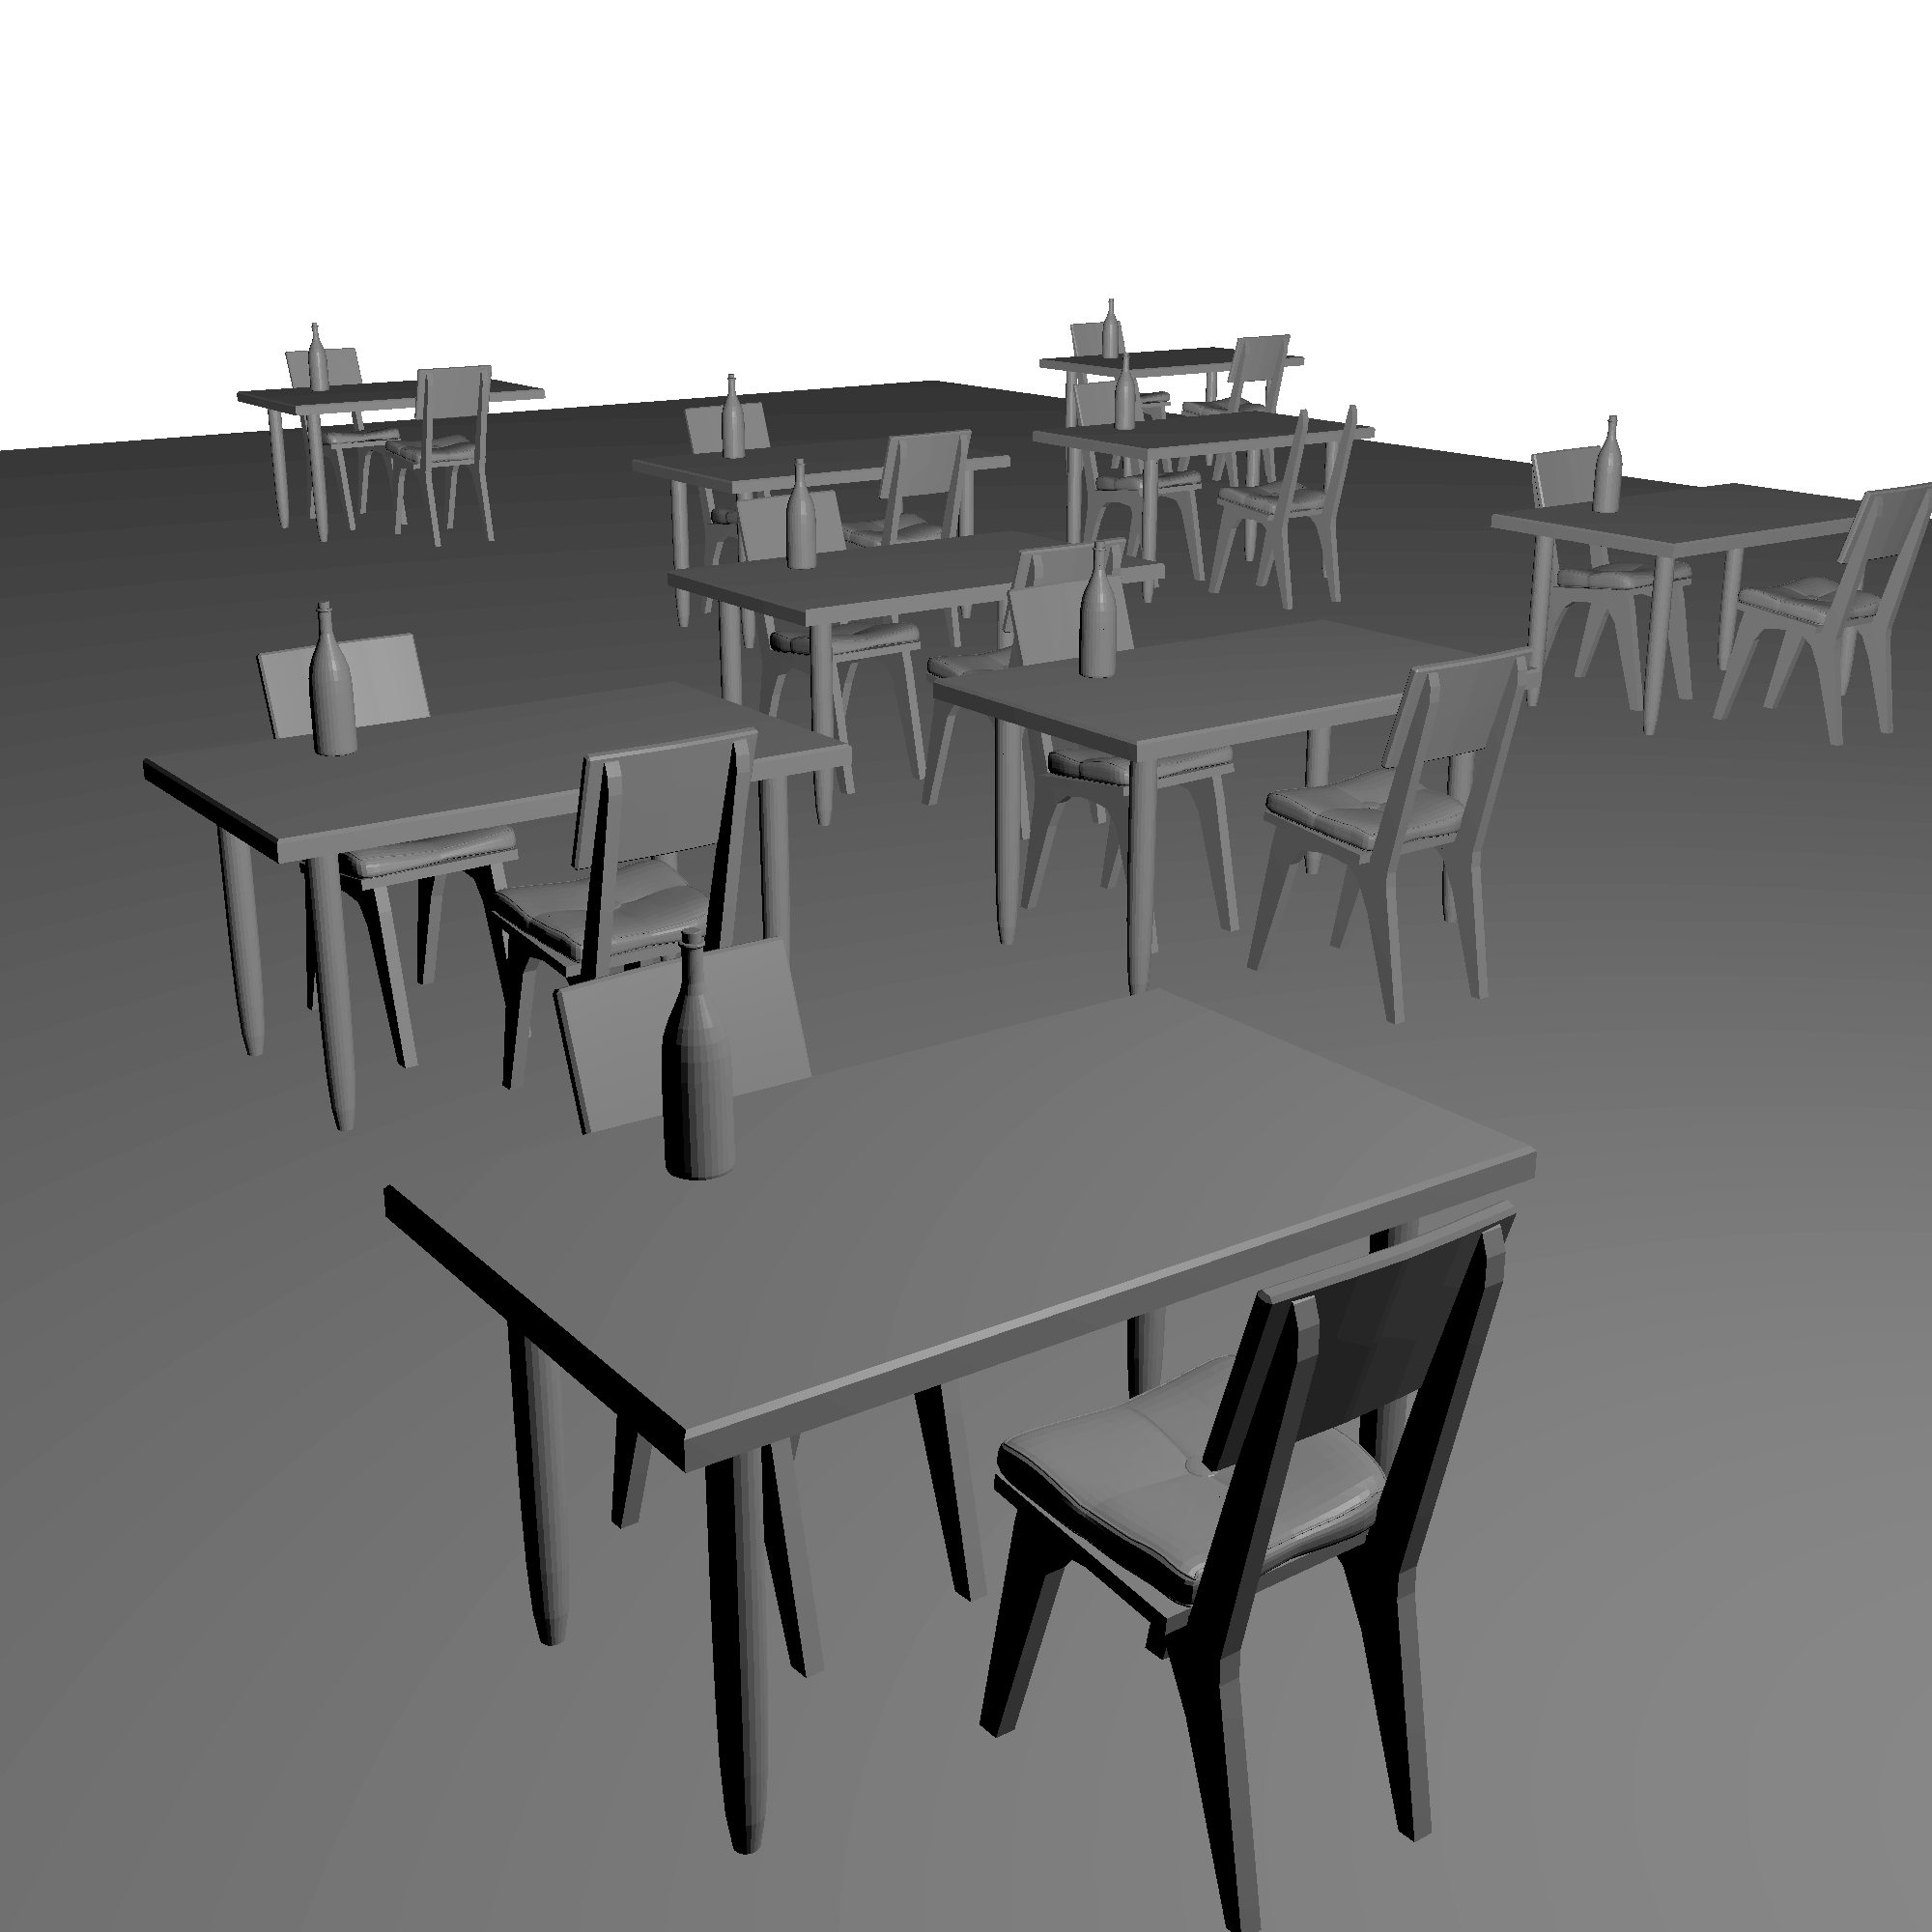
\includegraphics[width=\linewidth]{several_kitchen.png}
  \caption{Scene 2 with the tables}\label{fig:tables}
\endminipage
\minipage{0.3\textwidth}
  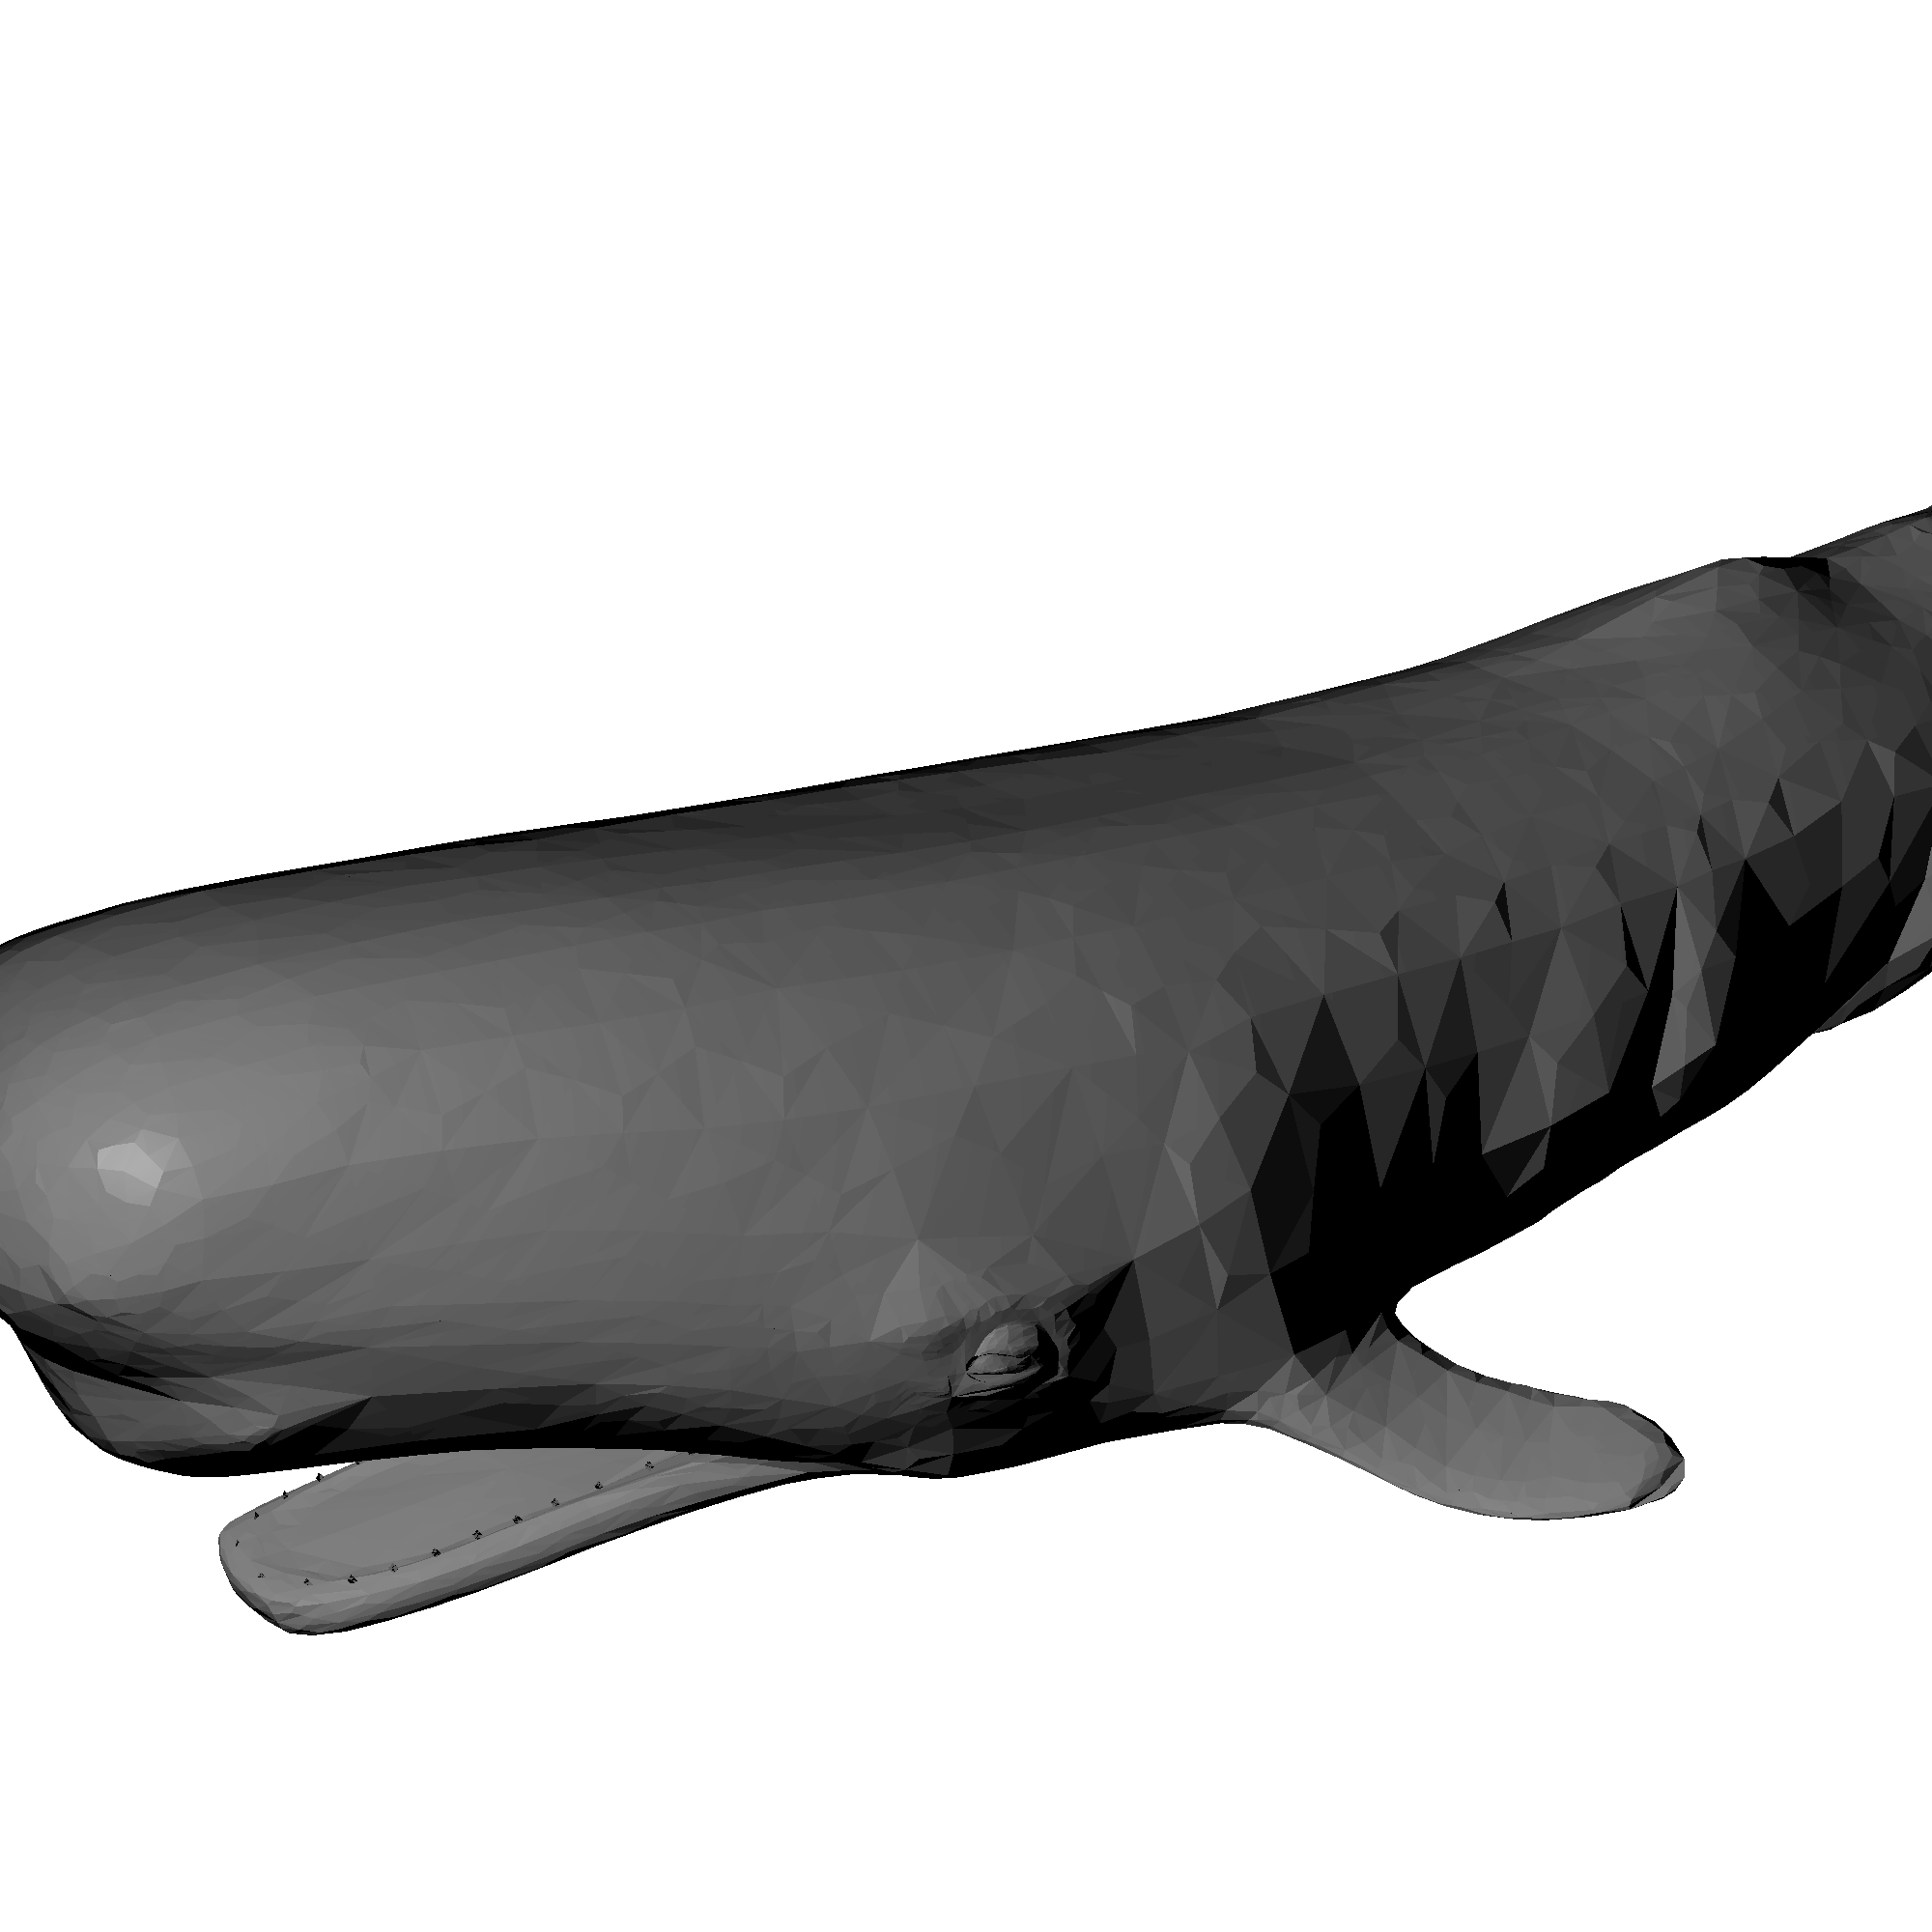
\includegraphics[width=\linewidth]{whale.png}
  \caption{Scene 3 with the single whale object}\label{fig:whale_scene}
\endminipage
\minipage{0.3\textwidth}%
  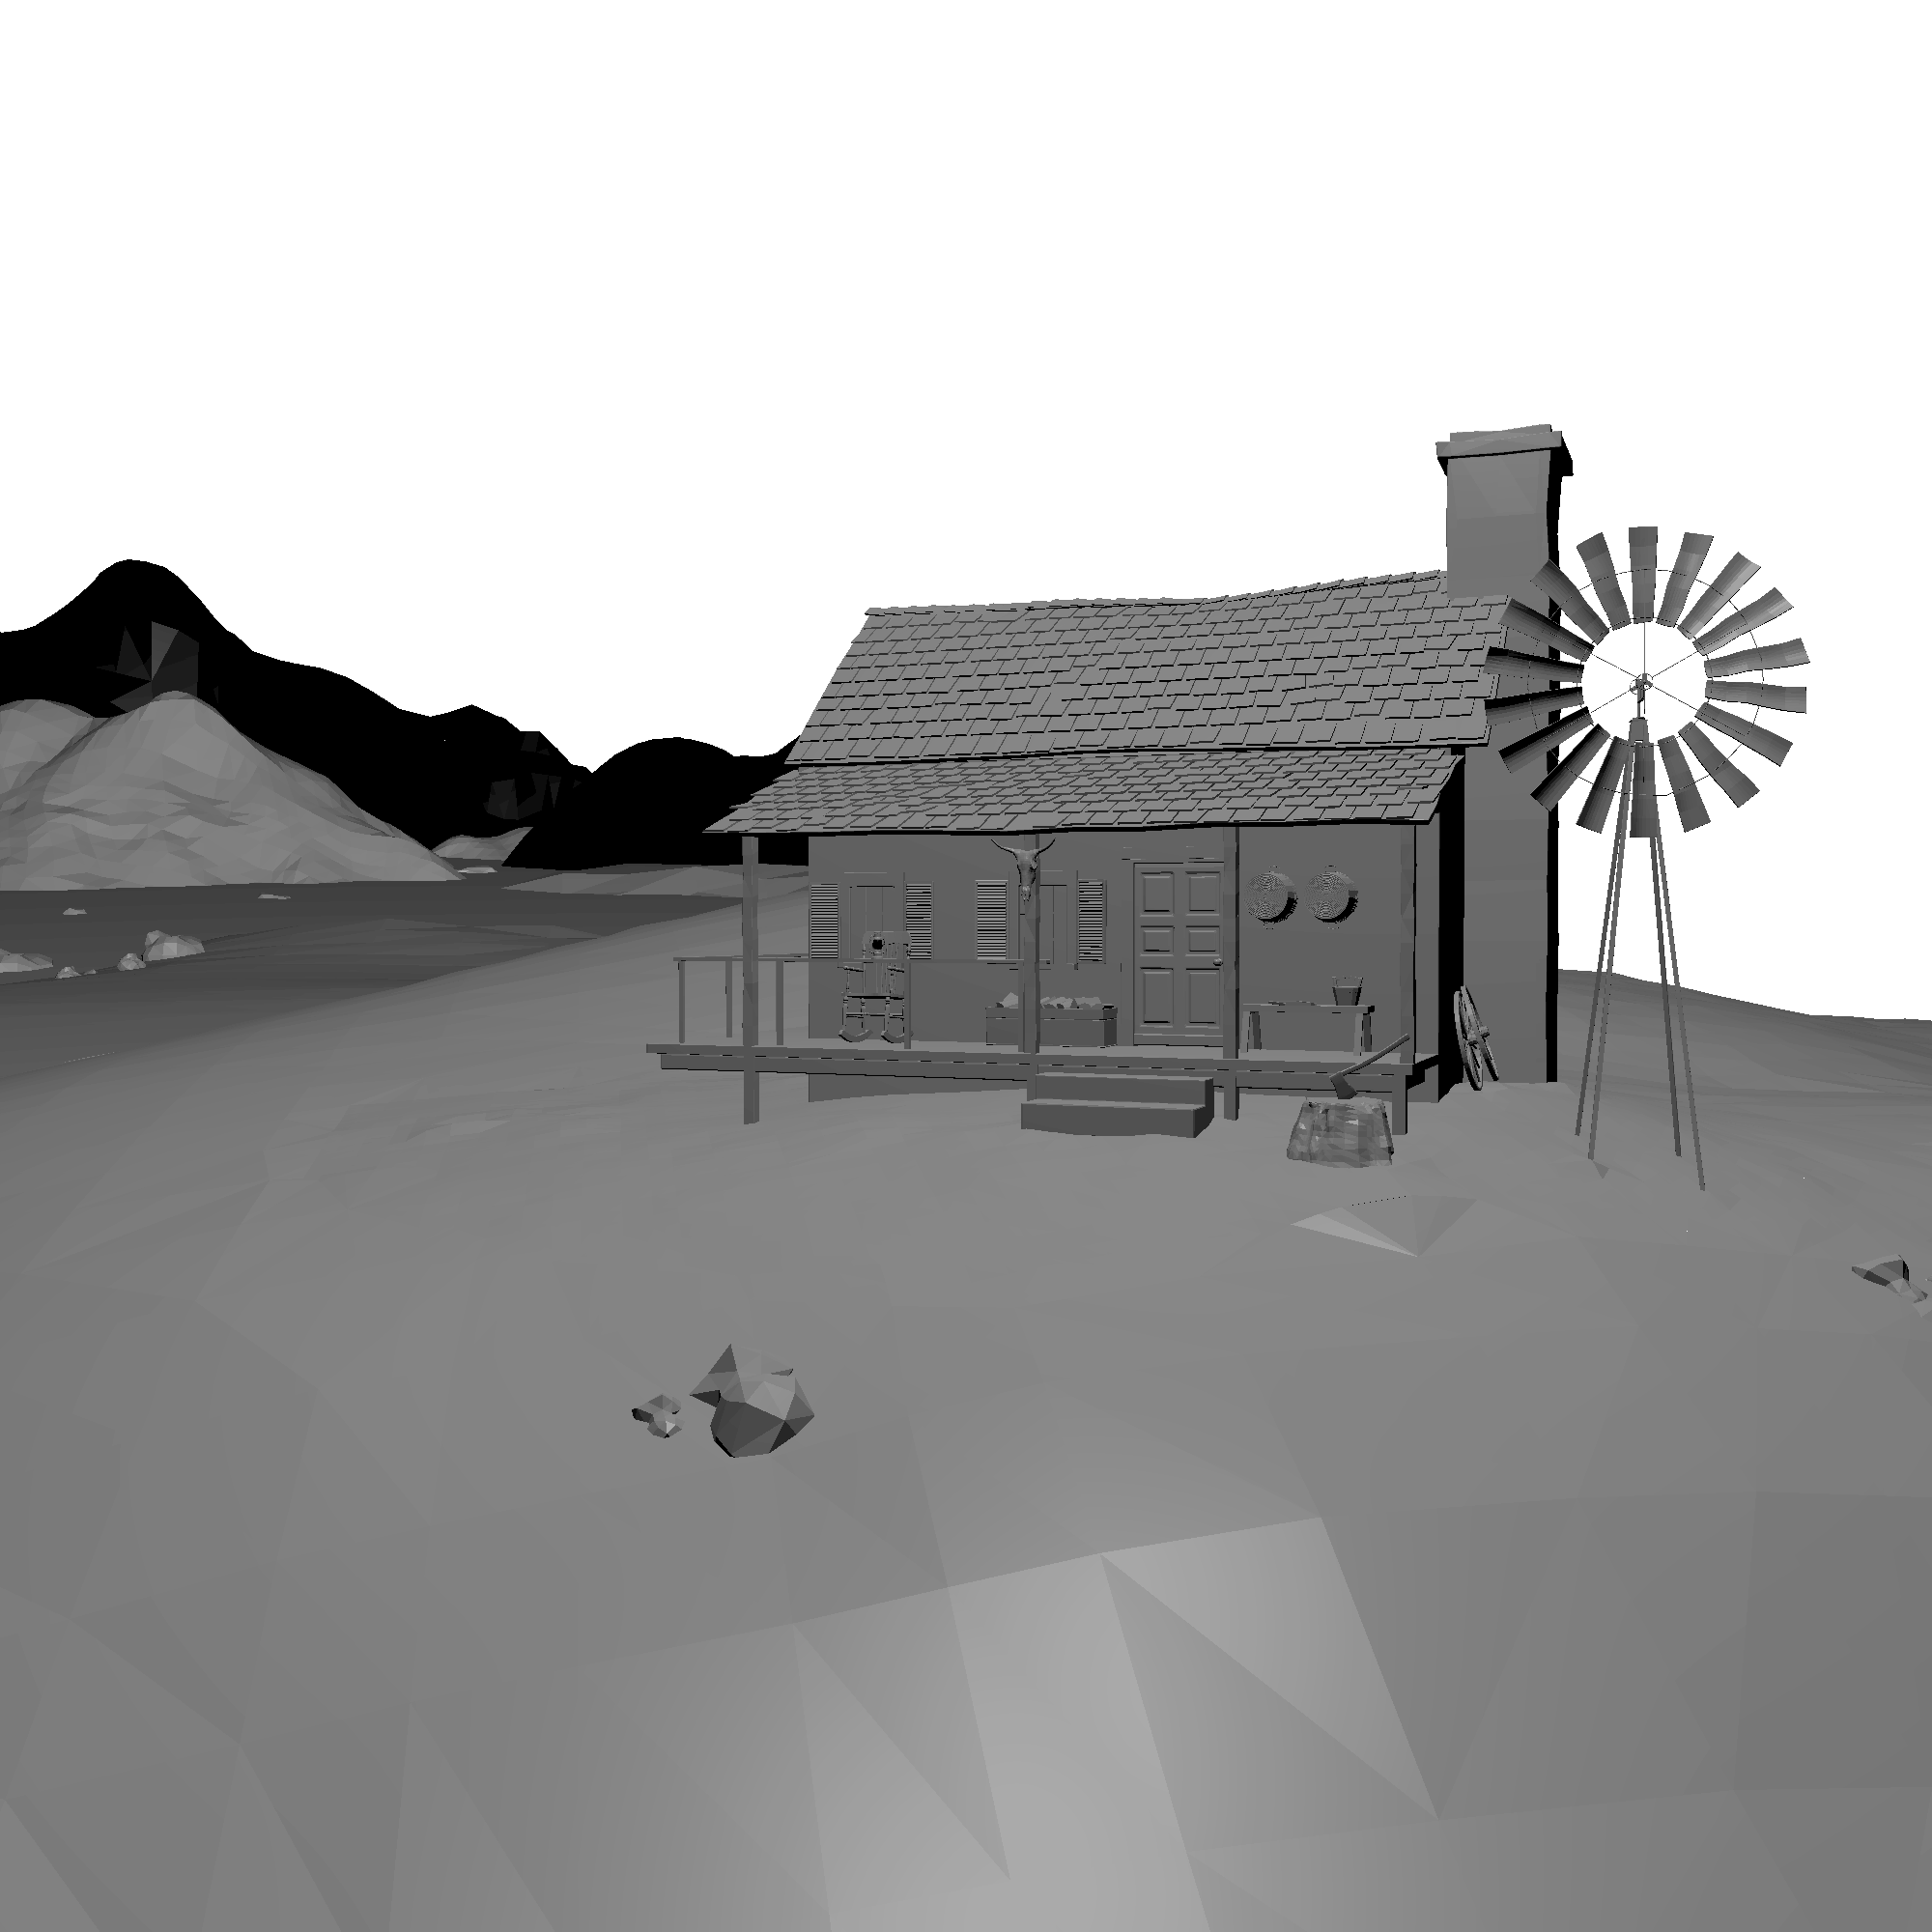
\includegraphics[width=\linewidth]{cabin.png}
  \caption{Scene 4 with the cabin}\label{fig:cabin_scene}
\endminipage
\end{figure*}

\begin{itemize}
\item Scene 1: A simple scene depicting a table and some kitchen
  objects. It contains 21.424 vertices, 42,848 triangles divided into
  28 objects.
\item Scene 2: The same scene as before but with several evenly
  distributed tables. It contains 203.644 vertices, 405.242 triangles
  divided into 233 objects. See figure~\ref{fig:tables}.
\item Scene 3: A scene with a single whale object containing 8.432
  vertices and 16.764 triangles. See figure~\ref{fig:whale_scene}.
\item Scene 4: A scene depicting a cabin. It contains 93.570 vertices,
  178.104 triangles divided into 250 objects. See
  figure~\ref{fig:cabin_scene}.
\end{itemize}

The figure~\ref{fig:scenes-results} shows ours results using the
scenes described previously. All tests were executed on a NVIDIA GeForce GTX
970 using driver version 353.30. The OpenCL specification
version used by this driver is 1.2.

\begin{figure}
\centering
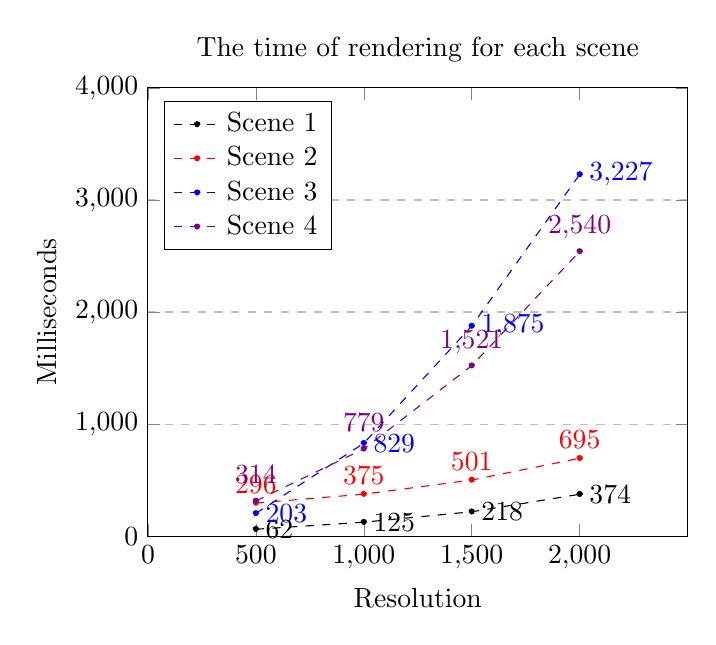
\begin{tikzpicture}
\begin{axis}[
    title={The time of rendering for each scene},
    xlabel={Resolution},
    ylabel={Milliseconds},
    xmin=0, xmax=2500,
    ymin=0, ymax=4000,
    xtick={0, 500,1000,1500,2000},
    ytick={0,1000,2000,3000,4000},
    legend pos=north west,
    ymajorgrids=true,
    grid style=dashed,
    scaled ticks=false, tick label style={/pgf/number format/fixed},
    legend entries={Scene 1, Scene 2,Scene 3,Scene 4},
]
% scene 1
\addplot[
    color=black,mark=*,mark size = 1, dashed, nodes near coords, nodes near coords align={horizontal}]
    coordinates {(500,62)(1000, 125)(1500,218)(2000,374)};
% scene 2
\addplot[color=red,mark=*,mark size = 1,dashed,nodes near coords]
    coordinates {(500,296)(1000, 375)(1500,501)(2000,695)};
%scene 3
\addplot[color=blue,mark=*,mark size = 1,dashed,nodes near coords, nodes near coords align={horizontal}]
    coordinates {(500,203)(1000, 829)(1500,1875)(2000,3227)};
% scene 4
\addplot[color=violet,mark=*,mark size = 1,dashed,nodes near coords=\raisebox{0.1cm}{\pgfmathprintnumber\pgfplotspointmeta}]
    coordinates {(500,314)(1000,779)(1500,1521)(2000,2540)};

\end{axis}
\end{tikzpicture}
\caption{Rendering time of the four scenes across different
  resolutions. Resolution value represents both width and height.}
\label{fig:scenes-results}
\end{figure}

From the graph we can see that the BVH works well with scenes that are
already divided into several objects. Scene 1 and 2 are good fits for
the algorithm because most leaf nodes have a low amount of geometry,
and the increase of resolution plays little role in the rise of
time. We can observe that the single object scene does not perform as
well as the other two, since in scene 3 a single object holds all
geometry, so we can observe that the BVH has little to no improvement,
since all rays certainly hit the AABB covering the whale, and in the
end the GPU has to test against all the geometry of the object for
almost all rays. This is due to the fact that the BVH partitions
objects, but it does not split geometry, so it depends if the scene
is already well divided into suitable chunks. An object with a large
amount of triangles that covers most of the frame will certainly slow
down any rendering, even if the triangle count of the scene is
relatively low. Scene 4 also performs poorly even though it has a good
amount of objects, the reason for this is that we have a floor object
on the scene that contains a great amount of triangles and covers most
of the frame, creating a situation like the whale scene.

We also tested against RenderGirl prior the implementation of the BVH,
by using a scene with several copies of the "Suzanne" model that comes
with Blender, but only one within the reach of the camera, rendered
with 1500x1500 pixels of resolution. Each object has 968 triangles and
507 vertices. We then tested both with and without the BVH with a
different amount of objects, as shown in
graph~\ref{fig:bvh-no-bvh-results}. In all tests, only one object
visible.

\begin{figure}
\centering
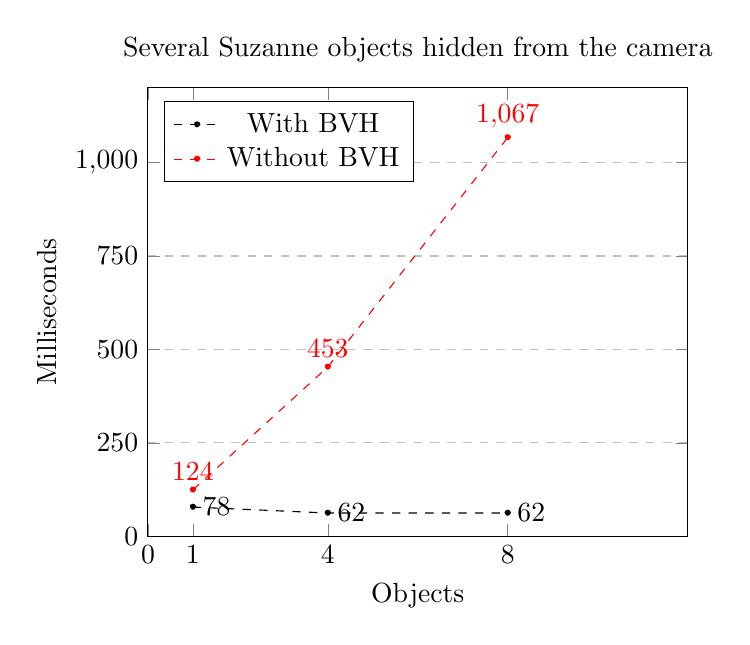
\begin{tikzpicture}
\begin{axis}[
    title={Several Suzanne objects hidden from the camera},
    xlabel={Objects},
    ylabel={Milliseconds},
    xmin=0, xmax=12,
    ymin=0, ymax=1200,
    xtick={0,1,4,8},
    ytick={0,250,500,750,1000},
    legend pos=north west,
    ymajorgrids=true,
    grid style=dashed,
    scaled ticks=false, tick label style={/pgf/number format/fixed},
    legend entries={With BVH , Without BVH},
]
\addplot[
    color=black,mark=* , mark size=1,dashed,nodes near coords,nodes near coords align={horizontal}
    ]
    coordinates {(1,78)(4, 62)(8,62)};
\addplot[
    color=red,mark=*, mark size = 1,dashed,nodes near coords
    ]
    coordinates {(1,124)(4, 453)(8,1067)};

\end{axis}
\end{tikzpicture}
\caption{Rendering time of three different scenes with a given amount
  of hidden objects. In all scenes, only one object is visible while
  the others are behind the camera.}
\label{fig:bvh-no-bvh-results}
\end{figure}

Based on graph~\ref{fig:bvh-no-bvh-results} we can notice that a brute
force approach forces the GPU to test against all geometry even if its
behind the camera, making a more steep time increase. Meanwhile the
BVH correctly ignore everything but the single object visible, so the
render time barely changes.

It was our intention to test the same scenes by rendering with and
without the BVH, but we discovered that the non-BVH version is not
capable of completing the render of scene 1, 2 and 4, crashing the
NVIDIA driver before finishing, and sometimes showing half-rendered
frames. This is likely because we enqueue a single kernel for the
whole frame. The limitation does not seem to arrive from lack of
memory, since both version have equal amount of memory consumption, so
we assume the driver does not properly schedule our command buffer,
and it is the application responsibility to make sure the kernel can
be enqueued at a given time.

For these results, we ignored the extra time spent on Python within
Blender, so all times are measurements from RenderGirl Core and not
from Blender. The Blender measurements are several seconds higher than
the Core. We attribute this to the slower nature of the Python
interpreter compared with native compiled code in C/C++. Also Blender
has to perform the triangulation of the entire scene and the data
structure conversion, which includes expensive division operations. We
don't think this undermine the results of the BVH and the raytracer as
whole, since we never focused our optimizations at this stage.


\section{Conclusions and future work}
\label{sec:conclusion}

The BVH performed well within the scope of its ability, providing good
speedups , even if with some known weaknesses of the acceleration
structure. For a future development, we could implement an hybrid of
kd-tree and BVH by partitioning objects that are above a given
threshold of triangle count, which would speed up cases like the whale
scene. Although we must still exercise caution on the complexity of
the partitioning scheme, since the generation of the structures are
done on the CPU side and it's serialized, while the traversal and ray
intersection operations takes full advantage of the OpenCL device. For
instance a BVH that takes 3 seconds more to generate must save at
least 3 seconds worth of processing on the device, so a solution for
the worst case of the BVH should taken into consideration the whole
context of the application.

The plugin architecture was validated by embedding the Core on three
different interfaces that can make use of the same library, e.g
Blender can run the unmodified RenderGirl that is also embedded on the
other two interfaces. We can also take advantage of all the facilities
Blender provides, such as image saving, 3D geometry loading and
triangulation features. This spare us of having to implement all from
scratch, enabling our work to be focused on the rendering
itself. However, we think more work is needed on the Python side of
RenderGirl, in order to reduce the extra seconds of delay we faced
when rendering scenes from within Blender.

Another welcome enhancement would be to dispatch the rendering into
several passes, which would likely solve the problem of the driver
crash in the non-BVH version of RenderGirl. In this approach a frame
could be divided into smaller frames, and each kernel enqueue would
render that specific sub-frame, until the full picture is generated.

With this work, we aim to offer more options for developers of 3D
modeling programs that want to incorporate a GPU raytracer into their
software without writing one from scratch.


% \section*{Acknowledgments}


\bibliographystyle{abbrv}
\bibliography{references}
\end{document}
